\documentclass[12pt]{article}
\usepackage[utf8]{inputenc}
\usepackage[spanish]{babel}
\usepackage{graphicx}
\usepackage{caption}
\usepackage{float}
\usepackage{amsmath}
\usepackage{geometry}
\geometry{margin=2.5cm}

\title{Resultados del Análisis y Optimización}
\author{}
\date{}

\begin{document}

\section*{4. Resultados}

La presente sección expone los principales hallazgos derivados del análisis de series temporales multivariadas y de la implementación de un modelo de optimización basado en programación lineal entera. El objetivo fue predecir la demanda semanal de seis productos esenciales y, con base en dichas predicciones, maximizar la rentabilidad de las compras respetando una restricción presupuestaria semanal.

\subsection*{4.1 Predicción de la demanda}

Posterior a la aplicacion del modelo ARX (AutoRegresivo con variables exógenas) para predecir la demanda de los productos: pan, pollo, arroz, huevo, detergente y shampoo. Las predicciones se realizaron sobre un horizonte de 22 semanas, utilizando los datos históricos de ventas correspondientes a las primeras 56 semanas como conjunto de entrenamiento. Las variables exógenas utilizadas fueron las ventas de los otros productos, bajo el supuesto de que podrían influir entre sí.

Para evaluar el desempeño del modelo en cada producto, se calcularon las métricas MAE (Error Absoluto Medio), RMSE (Raíz del Error Cuadrático Medio) y MAPE (Error Porcentual Absoluto Medio). Estas métricas indicaron niveles aceptables de precisión en la mayoría de los casos, lo cual respalda la viabilidad del modelo para estimar la demanda futura.
\begin{figure}[H]
    \centering
    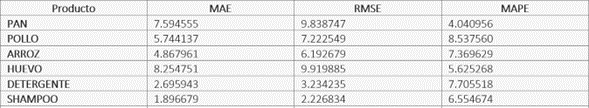
\includegraphics[width=0.8\textwidth]{error.png}
    \caption{MAE(Error Absoluto Medio), RMSE (Ráız del Error Cuadrático Medio) y MAPE (Error Porcentual Absoluto Medio)}
\end{figure}
Las visualizaciones correspondientes a cada producto mostraron una concordancia adecuada entre las series reales y las series predichas, lo que sugiere que el modelo logra capturar adecuadamente la tendencia y la estacionalidad de las ventas. En productos como el arroz y el pollo, la precisión fue mayor, mientras que en productos como el shampoo, las predicciones presentaron una mayor variabilidad.



\begin{figure}[H]
    \centering
    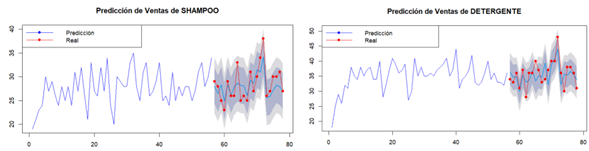
\includegraphics[width=0.8\textwidth]{Ima11.png}
    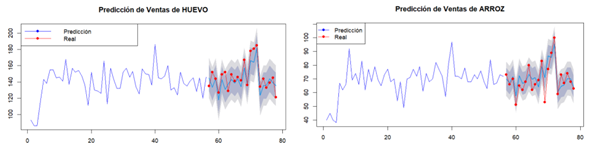
\includegraphics[width=0.8\textwidth]{Ima22.png}
    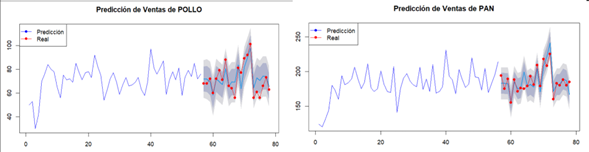
\includegraphics[width=0.8\textwidth]{Ima33.png}
    \caption{Predicción vs. datos reales para cada uno de los productos}
\end{figure}

\subsection*{4.2 Optimización de decisiones de compra}

Posteriormente, se procedió a optimizar las decisiones de compra semanales mediante la formulación de un problema de programación lineal entera (ILP). El objetivo de la optimización fue maximizar la ganancia semanal, definida como la diferencia entre el ingreso por ventas (precio de venta por unidad) y el costo de adquisición de cada producto.

Para cada semana, se impusieron dos restricciones:
\begin{itemize}
    \item Un límite presupuestario máximo de S/. 500.
    \item No exceder la cantidad predicha como demanda semanal.
\end{itemize}

Los resultados obtenidos evidencian una asignación eficiente del presupuesto semanal, priorizando productos con mayor rentabilidad relativa. El modelo permitió identificar, semana a semana, la combinación óptima de unidades a adquirir para cada producto, asegurando una utilización racional del presupuesto y un retorno económico favorable.


\begin{figure}[H]
    \centering
    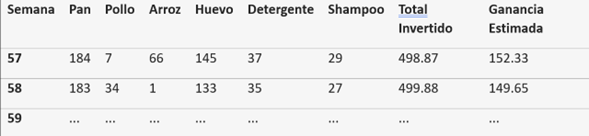
\includegraphics[width=0.75\textwidth]{tablaPRED.png}
    \caption{Resumen de compras óptimas y ganancias semanales (semanas 57–78)}
\end{figure}

\subsection*{4.3 Análisis visual de los resultados}

Se elaboraron visualizaciones que permiten observar de manera clara la evolución de los indicadores clave:

\textbf{Inversión y ganancia semanal (semanas 57–78):} La inversión se mantuvo cerca del límite presupuestal en la mayoría de las semanas, lo cual refleja un aprovechamiento casi completo del presupuesto disponible. En cuanto a la ganancia, esta se situó en un rango relativamente estable, con valores superiores a los S/. 150 por semana, alcanzando picos cercanos a S/. 190, dependiendo de la demanda proyectada y los márgenes de ganancia de los productos priorizados.

\begin{figure}[H]
    \centering
    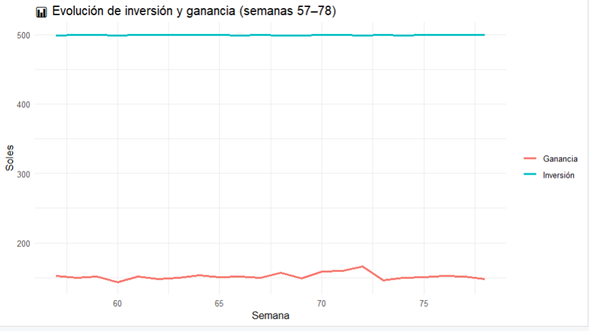
\includegraphics[width=0.75\textwidth]{Imagen3.png}
    \caption{Evolución de la inversión y ganancia semanal (semanas 57–78)}
\end{figure}

\textbf{Unidades adquiridas por producto:} El análisis gráfico de las cantidades compradas por semana mostró comportamientos diferenciados por producto. El pollo y el arroz, por su alto margen de ganancia y demanda estable, fueron adquiridos de forma constante. En contraste, productos como el shampoo y el detergente mostraron compras más intermitentes, influenciadas tanto por su demanda proyectada como por su menor rentabilidad relativa.

\begin{figure}[H]
    \centering
    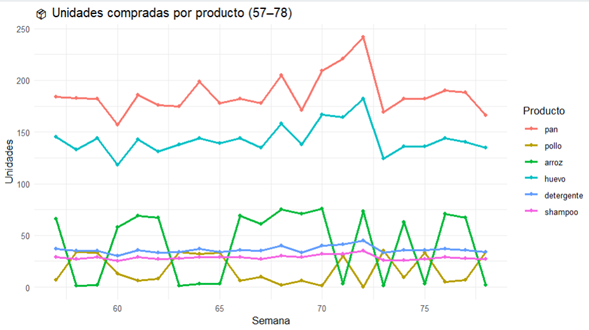
\includegraphics[width=0.8\textwidth]{uproducto1.png}
    \caption{Evolución semanal de unidades adquiridas por producto}
\end{figure}

Estos resultados reflejan el éxito del enfoque adoptado al integrar técnicas de predicción con métodos de optimización, proporcionando una herramienta efectiva para la toma de decisiones en contextos de planificación de inventarios bajo restricciones financieras.

\end{document}
